Схема распределения классов из модуля взаимодействия с пользователем по пакетам отображена на рис.~\ref{package_diagram_interaction}. Мы можем видеть, что отдельные пакеты отведены под классы, соответствующие различным элементам графического интерфейса (окна, вкладки и другие компоненты Swing), классы-контроллеры с бизнес-логикой приложения, классы, ответственные за реализацию паттернов проектирования <<Observer>> и <<Strategy>>, вспомогательные классы, а также под класс \texttt{Main} и класс для логирования. В этом разделе мы рассмотрим их подробно.

\begin{figure}[h]
\center{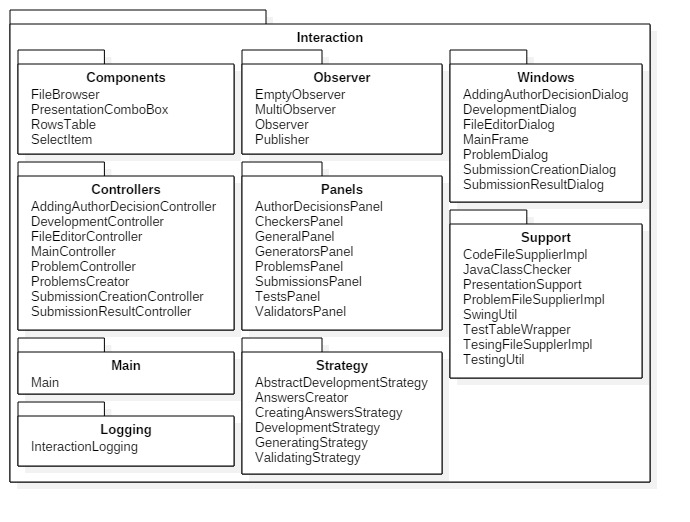
\includegraphics[scale=0.75]{package_diagram_interaction}}
\caption{Модуль взаимодействия с пользователем}
\label{package_diagram_interaction}
\end{figure}

В данном модуле для соединения графического интерфейса, бизнес-логики и отображаемых данных используется принцип схемы MVC. Это означает, что все классы, являющиеся элементами графического интерфейса, не содержат никакого кода бизнес-логики, а только оповещают классы-контроллеры о действиях со стороны пользователя. Классы-контроллеры, в свою очередь, выполняя некоторую бизнес-логику, берут из модели (в роли которой выступает интерфейс \texttt{File\-Supplier}) некоторую информацию и передают в компоненты Swing для отображения.

Таким образом, в данном модуле реализуется паттерн проектирования <<Ob\-ser\-ver>>~\cite{gamma}. Каждый класс, представляющий собой диалоговое окно, реализует интерфейс \texttt{Publisher}, имеющий методы для подписки в него по определённым идентификаторам реализаций интерфейса \texttt{Observer}. Как только в окне наступает некоторое событие, вызывается метод \texttt{notify()} соответствующего наблюдателя, и событие обрабатывается. При этом наблюдатели оформляют подписку на этапе инициализации окна. По такому принципу работают все диалоговые окна приложения.

В стартовой точке приложения (в классе \texttt{Main}) создаётся экземпляр класса \texttt{Main\-Controller}, отображающий главное окно приложения \texttt{Main\-Frame}. В данном контроллере создаётся экземпляр класса \texttt{Problems\-Creator}, объединяющий в себе используемые повсюду в приложении объекты типов \texttt{Testing\-System} и \texttt{File\-Supplier}. Именно в данном классе инициализируются реализации этих интерфейсов. Из специального XML-дескриптора \texttt{creators-pa\-rams.xml} берутся два свойства: максимальное количество одновременно запущеных процессов в тестирующей системе и путь к папке в файловой системе для хранения иерархии папок.

Перечислим все окна, присутствующие в данном приложении.

\begin{itemize}
\item \texttt{MainFrame} "--- в этом окне отображаются глобальные списки сделанных посылок и созданных задач (на двух вкладках \texttt{Submissions\-Panel} и \texttt{Problems\-Panel}). Посылки можно перезапускать, а для каждой задачи "--- открывать диалог для редактирования. 
\item \texttt{ProblemDialog} "--- диалоговое окно редактирования одной задачи. Присутствует шесть вкладок: для изменения общей информации о задаче (\texttt{General\-Panel}), тестов (\texttt{Tests\-Panel}), генераторов (\texttt{Generators\-Panel}), валидаторов (\texttt{Validators\-Panel}), чекеров (\texttt{Checkers\-Panel}) и авторских решений (\texttt{Author\-Decisions\-Panel}).
\item \texttt{FileEditorDialog} "--- окно для просмотра содержимого файла. Может открываться в двух режимах: только для чтения или для редактирования. Используется для просмотра входных и выходных данных тестов и исходного кода.
\item \texttt{DevelopmentDialog} "--- окно для вывода результатов работы генератора или валидатора, а также "--- процесса создания ответов на тесты.
\item \texttt{AddingAuthorDecisionDialog} "--- окно для выбора параметров нового авторского решения.
\item \texttt{SubmissionCreationDialog} "--- окно для выбора параметров новой посылки.
\item \texttt{SubmissionResultDialog} "--- окно с выводом полных результатов посылки или авторского решения на каждом тесте.
\end{itemize}

Заметим, что для реализации работы контроллера \texttt{Development\-Controller} был применён паттерн проектирования <<Strategy>>~\cite{gamma}, позволивший задавать контроллеру ожидаемое поведение. Для этого был отведён пакет с набором стратегий: для запуска генератора, валидатора и процесса создания ответов на тесты.

Также в отдельный пакет были вынесены некоторые дополнительные компоненты Swing, которых не хватало в самой библиотеке. Это, к примеру, текстовое поле, совмещённое с кнопкой <<Browse>> для автоматизированного ввода пути к файлу, и выпадающий список с поддержкой сопоставления каждому значению из списка некоторого удобочитаемого отображения в виде строки.

И, наконец, есть пакет со всеми вспомогательными классами, необходимыми в том числе для связывания воедино всех остальных модулей. Здесь находятся реализации интерфейсов из модуля тестирования, делегирующие выполнение интерфейсу \texttt{File\-Supplier}; классы \texttt{Swing\-Util} и \texttt{Testing\-Util}, реализующие некоторые типичные операции; класс \texttt{Java\-Class\-Checker}, позволяющий проверять ответ участника с помощью класса чекера, загруженного во время выполнения; класс \texttt{Test\-Table\-Wrapper} для облегчения работы с группами тестов; и класс \texttt{Presentation\-Support} с методами для определения визуального представления некоторых строковых идентификаторов.